\section{Problem Statement}

Mobile robots have widespread applications in industrial inspection, terrestrial and extraterrestrial exploration, and search and rescue missions. Wheeled or tracked systems are the most prevalent types of mobile robots that are being used for these tasks \cite{IntroductionAutonomousMobile}. Such robots typically adapt to changes in terrain through passive mechanical feedback \cite{belterAdaptiveMotionPlanning2016} and require a continuous path of support with minimal obstructions \cite{raibertLeggedRobotsThat1986} which restricts the kind of environments such systems can tackle to a minority of Earth's total landmass \cite{raibertBigDogRoughTerrainQuadruped2008}. Several critical environments, such as caves, forests, collapsed buildings, etc, pose challenges to these systems or render them entirely unusable. At the same time, these environments' terrain pose little challenge to animals, particularly ones that use legs for locomotion. Inspired from such animals, legged robots are an alternative category of mobile robots that are highly attractive due to their ability to traverse challenging terrain. Unlike wheeled or tracked systems that require a long patch of unobstructed terrain, legged robots only require isolated footholds to be unobstructed, greatly increasing their versatility in highly cluttered environments and rough terrain. Furthermore, they can climb over obstacles or squeeze through tight gaps by changing their morphology, similar to legged animals.

The current state-of-the-art robots such as Boston Dynamics' Spot \cite{Spot}, ANYBotics' ANYmal \cite{hutterANYmalHighlyMobile2016}, and Unitree's Go Series quadrupeds are used for assisting or even replacing humans in a variety of tasks due to their impressive locomotion capabilities \cite{SpotRescue, SpotRobotAssists, boumanAutonomousSpotLongRange2020, NovoNordiskExplores, gehringANYmalFieldSolving2021, tranzattoCERBERUSAutonomousLegged2022, hoellerANYmalParkourLearning2023, UnitreeFirefightingRobots2025}. Such high-end systems cost thousands of dollars \cite{kimPADWQDesignControl2021} due to expensive actuators, sensors, and compute modules.

We define, therefore, the problem statement of this capstone project as follows: 

\textit{How can we make a low-cost quadruped capable of traversing rough terrain in a purely proprioceptive manner? Furthermore, if we simulate a massless depth camera on the robot, how can we make the robot capable of navigating confined spaces using perception-based locomotion?}

\section{Proposed Solution}

We use a hobbyist robot kit, a Lynxmotion T-Hex 3DoF Hexapod repurposed into a quadruped, in order to demonstrate an inexpensive yet effective alternative for such robots. Our vision is that the robot, with teleoperation, would be able to handle varied rough terrain in real life while extending its behavior to perceive close environments using a camera and adapt its posture to minimize collisions while maintaining consistent and safe locomotion. Aside from proving that our locomotion pipeline is capable of working in even hobby-grade robots with adequate results, our proposed pipeline remains agile, versatile, and capable of further research and specialization for use cases such as search-and-rescue, cave exploration, and sundries.

\section{Intended User}

Our robotics systems's intended primary users are: researchers on robotics, academic developers, and operators looking for teleoperable platforms capable of exploring rough, confined environments such as subterranean caves, collapsed buildings, mountains, hazardous zones in construction, and so on.

\section{Project Gantt Chart and Deliverables}


\subsection{Kaavish I}
\begin{enumerate}
    \item Adopting the existing hardware and making the robot walk on flat ground. This includes:
    \begin{itemize}
        \item Re-assembling the robot to ensure proper orientation of motors. The robot was assembled by someone from EE 2023, and we cannot simply trust that it was assembled properly as improper assembly can result in having invalid commands to the motors causing irreparable damage
        \item Interfacing the motor controller with a Raspberry Pi 4. The current microcontroller for the robot is outdated and is not suitable for the tasks we intend to execute on the robot. As such, we will replace it with a Raspberry Pi 4 and interface that with the existing motor controller
        % \item Statistical analysis of the motors for better repeatability. The servo motors used in the legs do not have a readable angle output; for precise control, we would need to model the inaccuracy of each servo reaching a commanded position and incorporate that in our control strategies
        % \item Building a battery for the robot as per power requirements, keeping in mind future additions 
        \item Integrating all the hardware all together and implementing a basic gait. This gait does not need to be able to deal with rough terrain, it will simply be obtained from the kinematic model of the robot and is intended to make the robot walk on flat ground
    \end{itemize}
    \item Building the simulation model for the robot as well as the simulation environment. This includes:
    \begin{itemize}
        \item Identifying a suitable simulation environment. To ensure accurate simulation of locomotion strategies, a high fidelity physics engine like MuJoCo could be suitable; however, other considerations include integration with ROS and the ability to import custom models and environments
        \item Making a 3D model of the robot. The Lynxmotion website provides \texttt{sldprt} files that can be converted to \texttt{stp} files that can then be modified if needed and imported into any simulation software
        \item Identifying the parameters for the lava tubes terrain and scaling them down appropriately. 
        \item Making a simulation environment for testing. This can be handcrafted based on the parameters identified, but procedural random generation will allow for the robot to be extensively tested in simulation with better generalization and there is some recent work that suggests this could be possible \cite{garciaPLUMEProceduralLayer2025}
    \end{itemize}
    \item Extensive literature review of locomotion strategies, with some selected to be tested for the robot. The strategies will be selected based on a number of considerations, including the incorporation of feedback (open-loop vs closed-loop), novelty, and proven success. We will ensure that the selected strategies stretch across a number of paradigms, e.g. evolutionary algorithms, model-based RL, model-free RL etc.
    \item Literature review and initial implementation of multi-elevation mapping techniques. This includes:
\begin{itemize}
    \item Studying robot-centric mapping approaches and their application to confined space navigation \cite{buchananWalkingPostureAdaptation2019, mikiLearningRobustPerceptive2022}
    \item Implementing basic distance sensor data processing for multi-elevation map generation
    \item Developing algorithms to identify spatial constraints from sensor data
    \item Testing perception algorithms in simulation environment
\end{itemize}
\end{enumerate}

\subsection{Kaavish II}

\begin{enumerate}
    \item Modifications to the hardware to facilitate locomotion. This includes adding proprioceptive sensors to obtain feedback.
    \item Implementing the identified locomotion strategies in simulation.
    \item Implementing and testing the multi-elevation mapping system in simulation, integrating it with locomotion planning algorithms.
    \item Building the physical test environment for the robot.
    \item Deploying the locomotion strategies onto the physical robot and adjusting based on observed behavior. Locomotion controllers may need to be retrained with different constraints based on the behavior observed on the physical robot.
    % \item Deploying the perception system onto the physical robot and calibrating sensors for accurate spatial constraint detection.
\end{enumerate}


\begin{figure}[h!]
    \centering
    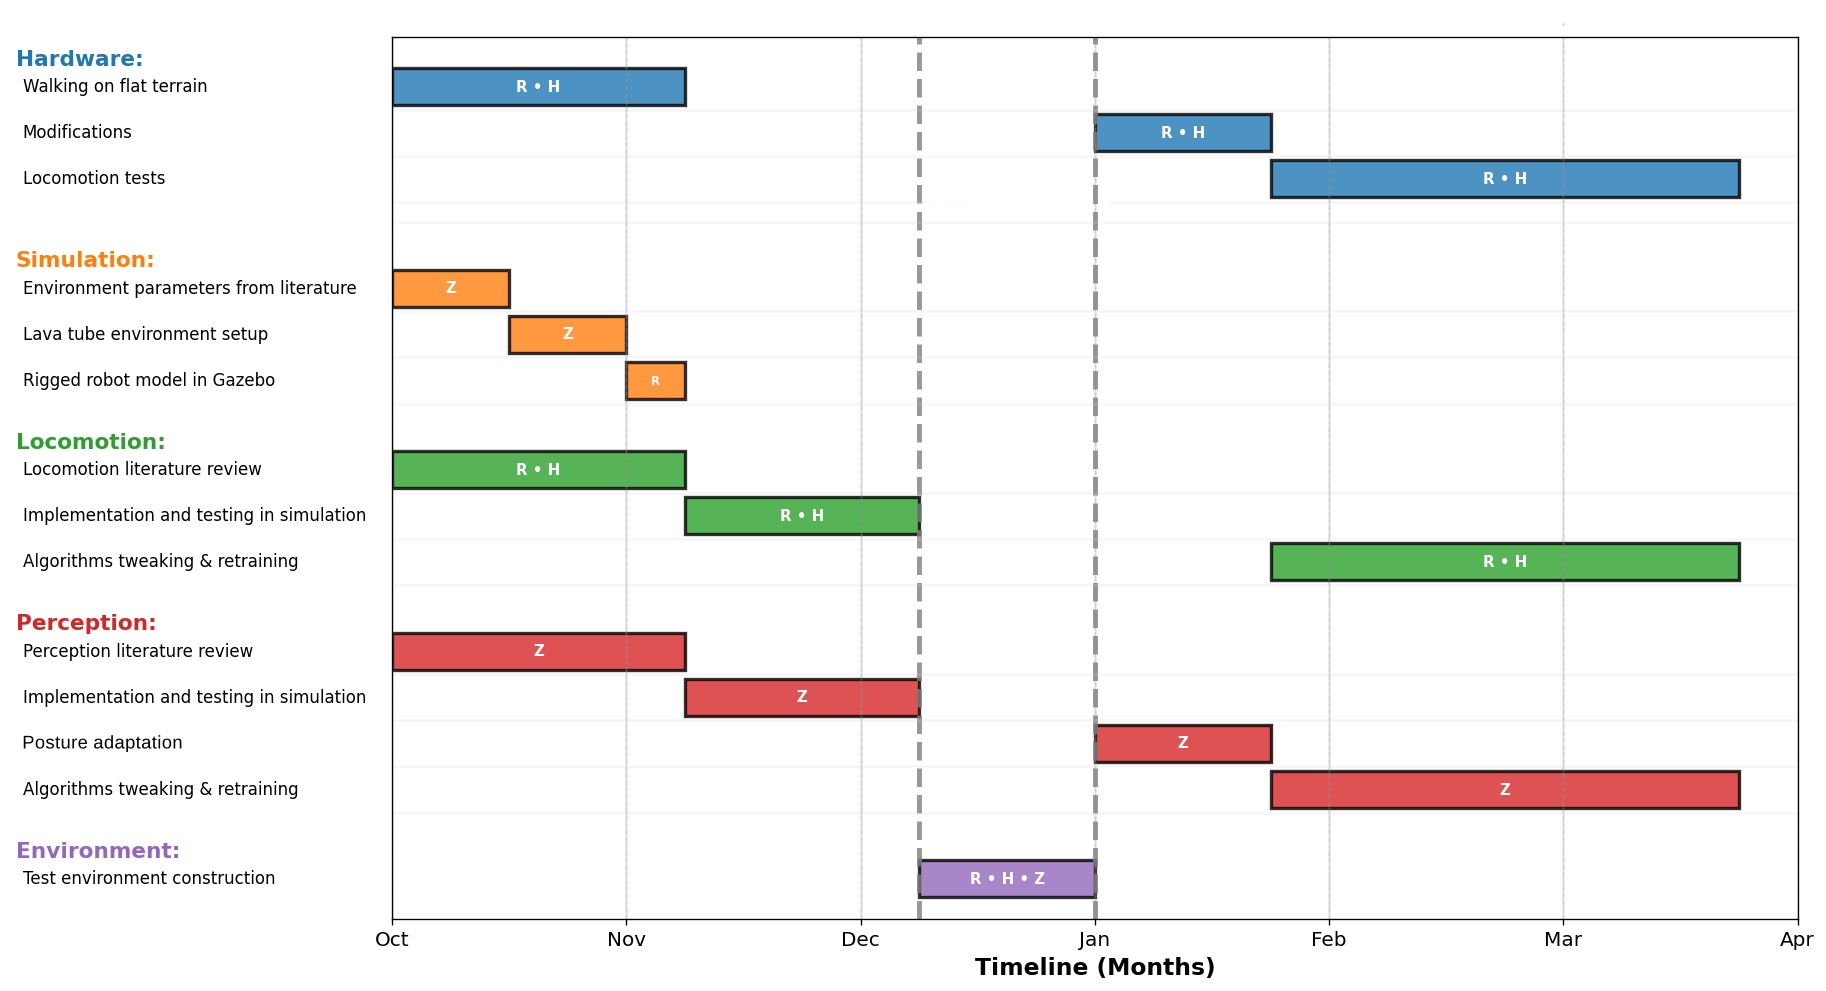
\includegraphics[width=1.0\textwidth]{gantt.png}
    \caption{The Gantt chart for scheduling tasks per team member.}
    \label{fig:gantt}
\end{figure}



\section{Key Challenges}

The project is highly constrained by the hobby-grade hardware. Key challenges include:
\begin{itemize}
    \item \textbf{Actuation Limits:} The motors are really weak as compared to other robots, even ones of the same size, thus making it much harder to put load on the robot or expect it to perform well. This plays a part in simulation as well as we try to accurately model the motor limits.
    \item \textbf{Power Constraints:} Making the robot stand draws 2A of current per side. Each power rail on our SSC-32U servo controller is rated for a maximum of 3A, leaving a critically narrow margin for dynamic movements.
    \item \textbf{Sim-to-Real Gap:} The robot does not have any proprioceptive sensors, so we had to retrofit an IMU and tap the potentiometers for joint state feedback. While these solutions are the most sensible out of everything we could do, this does introduce challenges as the feedback from the sensors is noisy and requires additional work to filter out noise.
    \item \textbf{Novelty of Posture Adaptation:} This is a significantly unexplored topic with approaches most often targetting posture adaptation for flat terrain, so concocting a personal approach deviating from literature is required here. 
\end{itemize}